\documentclass[12pt, twoside]{article}
\documentclass[12pt, twoside]{article}
\usepackage[letterpaper, margin=1in, headsep=0.2in]{geometry}
\setlength{\headheight}{0.6in}
%\usepackage[english]{babel}
\usepackage[utf8]{inputenc}
\usepackage{microtype}
\usepackage{amsmath}
\usepackage{amssymb}
%\usepackage{amsfonts}
\usepackage{siunitx} %units in math. eg 20\milli\meter
\usepackage{yhmath} % for arcs, overparenth command
\usepackage{tikz} %graphics
\usetikzlibrary{quotes, angles}
\usepackage{graphicx} %consider setting \graphicspath{{images/}}
\usepackage{parskip} %no paragraph indent
\usepackage{enumitem}
\usepackage{multicol}
\usepackage{venndiagram}

\usepackage{fancyhdr}
\pagestyle{fancy}
\fancyhf{}
\renewcommand{\headrulewidth}{0pt} % disable the underline of the header
\raggedbottom
\hfuzz=2mm %suppresses overfull box warnings

\usepackage{hyperref}
\usepackage{float}

\fancyhead[LE]{\thepage}
\fancyhead[RO]{\thepage \\ First and last name: \hspace{2.5cm} \,\\ Section: \hspace{2.5cm} \,}
\fancyhead[LO]{BECA/Huson/Geometry: Construction \\* 10 October 2024}

\begin{document}
\subsubsection*{1.23 Midterm Exam: Constructions \& transformations}
\begin{enumerate}[itemsep=0.5cm]
\item Construct an equilateral triangle with one side $\overline{AB}$.  
  \vspace{5cm}
  \begin{center}
  \begin{tikzpicture}
    \draw [-, thick] (0,0)--(5,1);
    \draw [fill] (0,0) circle [radius=0.05] node[below]{$A$};
    \draw [fill] (5,1) circle [radius=0.05] node[below]{$B$};
  \end{tikzpicture}
  \end{center}

\item Construct an angle bisector of the given angle.
  \vspace{3cm}
  \begin{center}
  \begin{tikzpicture}
    \draw [<->, thick] (-7,2)--(0,0)--(0.5,7);
    %\draw [fill] (0,0) circle [radius=0.05] node[below]{$A$};
  \end{tikzpicture}
  \end{center} \vspace{1cm}

\newpage
\item Construct a perpendicular bisector of $\overline{PQ}$.  
  \vspace{4cm}
  \begin{center}
  \begin{tikzpicture}
    \draw [-, thick] (0,0)--(5,-2);
    \draw [fill] (0,0) circle [radius=0.05] node[below]{$P$};
    \draw [fill] (5,-2) circle [radius=0.05] node[below]{$Q$};
  \end{tikzpicture}
  \end{center} 
  \vspace{3cm}

\item Construct a perpendicular to line $l$ through the point $P$.  
    \vspace{4cm}
    \begin{center}
    \begin{tikzpicture}
        \draw [<->, thick] (0,0)--(10,-5) node [below right]{$l$};
        \draw [fill] (4.5,0) circle [radius=0.05] node[below right]{$P$};
    \end{tikzpicture}
    \end{center}

\newpage
\subsubsection*{1.23 Midterm Exam: Transformations}
\item Translate $\triangle ABC$ left five and down three units. Label the image $\triangle A'B'C'$.
\begin{center}
    \begin{tikzpicture}[scale=0.7]
    \draw [help lines] (-8,-6) grid (8,6);
    \draw [thick, <->] (-8.4,0) -- (8.4,0) node [right] {$x$};
    \draw [thick, <->] (0,-6.4)--(0,6.4) node [above] {$y$};  
    \draw [thick]
      (3,4) node[above right] {$A$}--
      (3,-2) node[below] {$B$}--
      (6,3) node[below right] {$C$}--cycle;  
  \end{tikzpicture}
\end{center}

\item Reflect $\triangle DEF$ across the $x$-axis, labeling the image $\triangle D'E'F'$.
\begin{center}
    \begin{tikzpicture}[scale=.7]
    \draw [help lines] (-8,-6) grid (8,6);
    \draw [thick, <->] (-8.4,0) -- (8.4,0) node [right] {$x$};
    \draw [thick, <->] (0,-6.4)--(0,6.4) node [above] {$y$};  
    \draw [thick]
      (2,1) node[above left] {$D$}--
      (7,4) node[above right] {$E$}--
      (7,1) node[below right] {$F$}--cycle;  
  \end{tikzpicture}
\end{center}

\newpage
\item Rotate the triangle $90^\circ$ clockwise around the origin, $\triangle ABC \rightarrow \triangle A'B'C'$. Complete the table of the coordinates and plot and label the image on the grid. \vspace{0.5cm}
\begin{multicols}{2}
  $A(0,0) \rightarrow$ \\[0.7cm]
  $B(2,4) \rightarrow$ \\[0.7cm]
  $C(2,0) \rightarrow$ \\[0.7cm]
    \begin{tikzpicture}[scale=.70]
    \draw [help lines] (-5,-5) grid (5,5);
    \draw [thick, <->] (-5.4,0) -- (5.4,0) node [right] {$x$};
    \draw [thick, <->] (0,-5.4)--(0,5.4) node [above] {$y$};  
    \draw [thick]
      (0,0) node[below left] {$A$}--
      (2,4) node[above right] {$B$}--
      (2,0) node[above right] {$C$}--cycle;  
    \end{tikzpicture}
  \end{multicols}

\item Triangle $X'Y'Z'$ is the image of triangle $XYZ$ after a translation. Which triangle is larger, or are they the same size? Justify your answer. \vspace{3cm}

\item A reflection maps $P(-5,3)$ onto $P'(5,3)$. Is the reflection across the $x$-axis or the $y$-axis? \vspace{2cm}

\item Specify the translation that maps $Q(-1,2)\rightarrow Q'(6,-5)$.


\newpage
\item Simplify each expression by combining like terms.
  \begin{multicols}{2}
      \begin{enumerate}[itemsep=1.5cm]
        \item $7x+5-2x+3$
        \item $-5y^2-4y+8y+y^2$
        \item $5+5\pi+7-3\pi$
        \item $12x-7+4\sqrt{5}+2\sqrt{5}$
      \end{enumerate}
  \end{multicols} \vspace{1cm}

\item Use the function $f(x) = 8x-3$ to answer the questions.
  \begin{multicols}{2}
  \begin{enumerate}[itemsep=2cm]
      \item What is $f(0)$?
      \item Find $f(\frac{1}{4})$
      \item What is $x$ when $f(x) = 69$?
  \end{enumerate}
  \end{multicols} \vspace{2cm}

\item Solve each equation for $x$. Then check your answer.
  \begin{multicols}{2}
    \begin{enumerate}[itemsep=1cm]
  \item $2x+7x+13=31$
  \item $5x-7=8x+14$
  \end{enumerate}
  \end{multicols}


\newpage
\item As shown below, two lines intersect making four angles: $\angle 1$, $\angle 2$, $\angle 3$, and $\angle 4$.
  \begin{multicols}{2}
    Given m$\angle 1 = 70^\circ$.  
    \begin{enumerate}
      \item Find m$\angle 3$ \vspace{2cm}
      \item Find m$\angle 4$ \vspace{2cm}
    \end{enumerate}
    \begin{tikzpicture}[scale=0.7, rotate=20]
    \draw[<->, thick] (0,-1.5)--(10,1.5);
    \draw[<->, thick] (2,3.5)--(7,-3.5);
    \node at (3,.4){1};
    \node at (6,-.6){3};
    \node at (5,1){2};
    \node at (4,-1){4};
  \end{tikzpicture}
  \end{multicols} \vspace{0.5cm}

\item Given that the $m \angle UST = 55^\circ$. Find the $m \angle RSU$
  \begin{center}
  \begin{tikzpicture}[scale=1.3]
    \draw[->, thick] (0,0)--(55:5);
    \draw[<->, thick] (-3,0)--(7,0);
    \draw[fill] (55:4) circle [radius=0.05] node[above left ]{$U$};
    \draw[fill] (-2,0) circle [radius=0.05] node[below]{$R$};
    \draw[fill] (0,0) circle [radius=0.05] node[below]{$S$};
    \draw[fill] (4,0) circle [radius=0.05] node[above]{$T$};
  \end{tikzpicture}
  \end{center}

\item Given two parallel lines, two transversals, and angle measures as marked.
\begin{multicols}{2}
  Find $x$, $y$, $z$

    \begin{tikzpicture}[scale=1.6]
    \draw [<->, thick] (4,2.25)--(7,2.25);
    \draw [<->, thick] (3.5,0)--(7,0);
    \draw [<->, thick] (4,-0.5)--(5.7,3);
    \draw [<->, thick] (6.5,-0.5)--(5,3);
    \node at (4.4,0.3) [right]{$69^\circ$};
    \node at (5.5,0.3) [right]{$86^\circ$};
    \node at (5.1,2.2) [below left]{$x^\circ$};
    \node at (5.35,1.9) [below]{$y^\circ$};
    \node at (5.5,2.2) [below right]{$z^\circ$};
  \end{tikzpicture}
\end{multicols}

\end{enumerate}
\end{document}